\chapter{\uppercase{Comparative Genomic Analysis of \emph{P. papatasi} and \emph{L. longipalpis} Sand Fly Genomes}}

\section{Introduction}
Cutaneous leishmaniasis infects the skin, causing painful sores which can reoccur up to 20 years after infection, even in individuals who have been adequately treated. The deadly form visceral leishmaniasis is the second-largest parasitic killer in the world, responsible for 200,000 to 400,000 infections per year worldwide; the largest being malaria.

Leishmaniasis is caused by protozoan parasites of the \emph{Leishmania} genus that are transmitted by phlebotomine sand flies. Phlebotomine sand flies are a diverse group of vectors that vary widely in geographic distribution, ecology, and the pathogens they transmit. Diversity in both the \emph{Leishmania} parasite and sand flies leads to complex parasite-vector interactions and emits parasite-vector specificity.

The interactions between the \emph{Leishmania} parasite and sand fly studies have been an area of significant study but multiple questions remain \cite{Dostalova2012}.  \emph{Leishmania} development largely takes place in the sand fly digestive tract. Digestion enzymes such as trypsins and chymotrypsins have been reported to destroy the parasites in ``incompatible'' sand fly species \cite{Pimenta1997}.  Peritrophic matrices are thought to protect the parasites from the digestion enzymes, while also trapping the parasites if the matrices are not broken down by chitinases \cite{Pimenta1997}.  Depletion of the Caspar negative immune system regulator has been observed to reduce infection rates in \emph{L. longipalpis} \cite{Telleria2012}.  Near the end of the digestion process, the \emph{Leishmania} parasites need to bind themselves to the sand flies' midgut epithelium to avoid being excreted with the blood remnant \cite{Pimenta1994}.  It must be emphasized that the interactions are not just one way; differences in  gene expression levels between infected and non-infected sand flies have been widely noted. 

The genomes of \emph{Phlebotomus papatasi} and \emph{Lutzomyia longipalpis} have recently been sequenced, offering opportunities to better understand the vector-parasite relationship through comparative analysis. \emph{P. papatasi} is found in the Old World, particularly Northern Africa and the Middle East. \emph{P. papatasi} is the major vector of cutaneous leishmaniasis, caused by \emph{L. major}.  \emph{L. longipalpis} is found in Latin America. \emph{L. longipalpis} transmits \emph{L. chagasi} / \emph{L. infantum}, which causes visceral leishmaniasi.

Here, we focus on a genomic comparison of \emph{P. papatasi} and \emph{L. longipalpis}, using the mosquitoes \emph{Ae. aegypti} and \emph{An. gambiae} and fruit flies \emph{D. melanogaster} and \emph{D. simulans} as controls.  We begin by analyzing completeness of the sand fly genome assemblies.  We follow with analysis of synteny, or conserved gene order, and $d_N$/$d_S$, the rate of non-silent substitutions to silent substitutions, distributions for single-copy orthologs.  We analyze differential gene expression in blood-fed, sugar-fed, and infected blood-fed \emph{L. longipalpis} females using RNASeq.  Lastly, we analyze the expression and synteny of peritrophins, chitinases, and Niemann-Pick type C-2 (NPC2) genes.

\section{Methods}

\subsection{Data sets}
The \emph{Ae. aegypti}, \emph{An. gambiae}, \emph{L. longipalpis}, and \emph{P. papatasi} \textcolor{red}{TODO VERSIONS} peptide translations were downloaded from Vectorbase \textcolor{red}{TODO CITE}, while the \emph{D. melanogaster} and \emph{D. simulans} peptide translations were downloaded from Flybase \textcolor{red}{TODO CITE}.

\textcolor{red}{table of versions and sources}

\subsection{Assembly Statistics}
Cumulative density function plots of the gene distributions over the scaffolds were generated as follows: The gene counts of each genome's scaffolds were normalized by dividing the gene counts by the number of genes in that organism's genome. For each genome, lists of the normalized gene counts were sorted largest to smallest and padded with 0-value entries so that all of the lists had the same length.  Cumulative sums were computed over the normalized gene counts and plotted.


\subsection{Synteny}
To generate the scatter plots, the identifiers, scaffolds, locations, and sense in the FASTA headers were extracted for each peptide sequence.  The protein IDs were cross-referenced with OrthoDB to group the proteins into ortholog groups.  Sequences without ortholog information or no orthologs in the other genomes and ortholog groups with many-to-many and one-to-many relationships were discarded.  The proteins were sorted along each scaffold by their starting coordinates, while scaffolds were ordered arbitrarily.  Scatter plots were generated by drawing dots at the positions of orthologous proteins.

Microsynteny blocks were identified using SynChro. For each genome, the identifiers, protein sequences, orientations, scaffolds, and locations extracted from FASTA files for each genome and reformatted as input for SynChro \cite{Drillon2014}.  SynChro ($\Delta=5$) was run on the pairs \emph{D. melanogaster} and \emph{D. simulans}, \emph{An. gambiae} and \emph{L. longipalpis}, \emph{An. gambiae} and \emph{Ae. aegypti}, and \emph{L. longipalpis} and \emph{P. papatasi}.  Three-way synteny blocks for \emph{An. gambiae}, \emph{L. longipalpis}, and \emph{P. papatasi} were constructed by finding all pairs of synteny blocks for \emph{An. gambiae} and \emph{L. longipalpis} and \emph{L. longipalpis} and \emph{P. papatasi} that overlapped by at least one gene.  

The top five largest (by counts of total genes) synteny blocks from selected from the \emph{L. longipalpis} and \emph{P. papatasi} and \emph{Ae. aegypti}, \emph{L. longipalpis}, and \emph{P. papatasi} comparisons.  Genes were annotated using BLAST against the NCBI nr database \cite{Pruitt2007}.

\subsection{$d_N$/$d_S$ Distributions}
Protein sequences were organized into ortholog groups according to OrthoDB v8 \cite{Kriventseva2015}. Groups that did not have at least one sequence from each species were discarded.  For groups with 1-to-many and many-to-many orthologs, one protein sequence was chosen randomly from each species with uniform weights. Protein multiple sequence alignments were generated using Clustal Omega \cite{Sievers2011} and used to inform CDS alignments with the codon-aware PAL2NAL alignment program \cite{Suyama2006}.  The yn00 program from PAML v4.8 \cite{Yang2007} was used to calculate $d_N$/$d_S$ ratios for each pairs of sequences in the aligned ortholog groups.

\subsection{RNASeq}
CuffDiff \cite{Trapnell2010} was used to identity genes with statistically-significient differences in expression levels between pairs of feeding conditions (sugar fed, blood fed, and infected blood fed) at each time point (6 h, 24 h, and 144 h after feeding).  BLAST2GO \cite{Conesa2005,Gotz2008} was used to assign GO-slim terms \cite{Consortium2004} to the corresponding peptide sequences for each gene. BLAST2GO's Fisher Exact Test analysis was used to test distributions of GO-slim terms from pairs of conditions (at the same time points) for statistically-significent differences.

Additionally, genes from manually-annotated families were analyzed.  Genes with marked as having statistically-differences in expression at two or time points were isolated.

\section{Results and Discussion}
We performed a comparative analysis of the genomes of two sand flies species \emph{L. longipalpis} and \emph{P. papatasi}, using comparisons with and between \emph{Ae. aegypti}, \emph{An. gambiae}, \emph{D. melonagaster}, and \emph{D. simulans} as controls.

\subsection{Genome Assembly Fragmentation}
Fragmentation of a genome assembly significantly effects comparative genomic analysis.  We analyzed and compared the distribution of genes across the scaffolds from the genomes of the sand flies \emph{P. papatasi} and \emph{L. longipalpis}, mosquitoes \emph{Ae. aegypti} and \emph{An. gambiae}, and fruit flies \emph{D. melonagaster} and \emph{Dr. simulans} (Figure~\ref{fig:scaffolds}).  The six organisms have between 10,100 and 17,294 genes.  Assemblies of the \emph{An. gambiae} and \emph{D. melonagaster} genomes are relatively complete and are used as our standard for comparison; both have one scaffold per chromosome with between 1,000 and 4,000 genes located on the five largest scaffolds.

The assembly of the \emph{D. simulans} genome is partially fragmented but still relatively complete.  The assembly has more scaffolds (1,131) than chromosomes, but sizes (in terms of genes) of the five largest scaffolds are comparable to \emph{An. gambiae} and \emph{D. melonagaster}.  Comparison of the cumulative distribution of gene locations from largest to smallest scaffolds suggests that a majority of \emph{D. simulans}'s genes are located on a small number of large scaffolds with about 10\% of the genes distributed across a number of small scaffolds.

Analysis of \emph{P. papatasi}, \emph{L. longipalpis}, and \emph{Ae. aegypti} suggest a different story, with high levels of fragmentation.  All three organisms have a large number of scaffolds (4,350, 1,928, and 1,633 scaffolds, respectively) and fewer than 100 genes are located on each of their five largest scaffolds (see Figure~\ref{fig:scaffolds}).  The cumulative distribution of genes indicates that the genes of \emph{P. papatasi} are nearly uniformly distributed across the scaffolds.  While not uniformally distributed, 90\% of the genes of \emph{L. longipalpis} and \emph{Ae. aegypti} are spread scross 1,000 scaffolds. The largest scaffolds of \emph{Ae. aegypti} (104 genes), \emph{L. longipalpis} (73), and \emph{P. papatasi} (84) are much smaller than the largest scaffolds sizes of \emph{D. melonagaster} (3,991 genes), \emph{D. simulans} (3,767 genes), and \emph{An. gambiae} (3,684) (see Table~\ref{tab:scaffold-sizes}). Fragmentation is not unexpected given the high rates of genome shuffling observed in comparative analyses of insect genomes \cite{Zdobnov2007,Ranz2001}.  High rates of genome shuffling may limit the utility of well-assembled genomes as references in the assembly process, further complicating the assembly process.


\begin{figure}[H]
  \centering
  \caption{GENOME ASSEMBLY STATISTICS}
  \begin{subfigure}[b]{0.45\textwidth}
    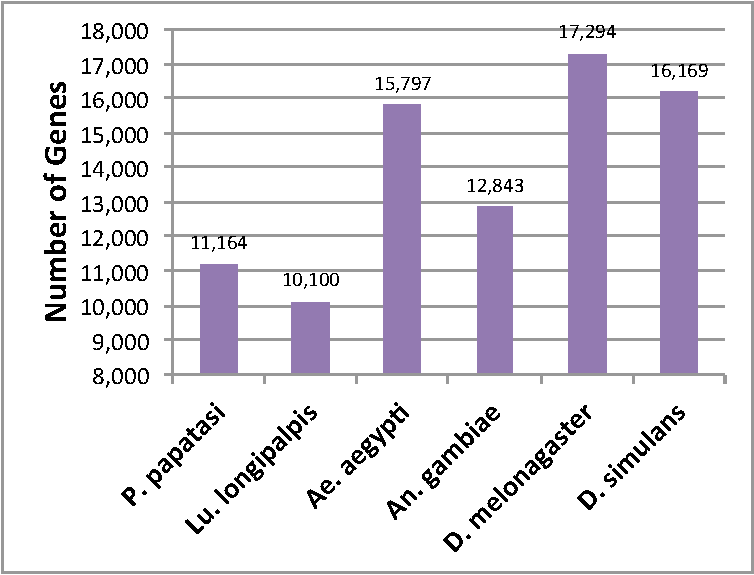
\includegraphics[width=\textwidth]{figures/synteny/genome_size_genes.pdf}
    \caption{Genome Sizes (Genes)}
  \end{subfigure}
  ~
  \begin{subfigure}[b]{0.45\textwidth}
    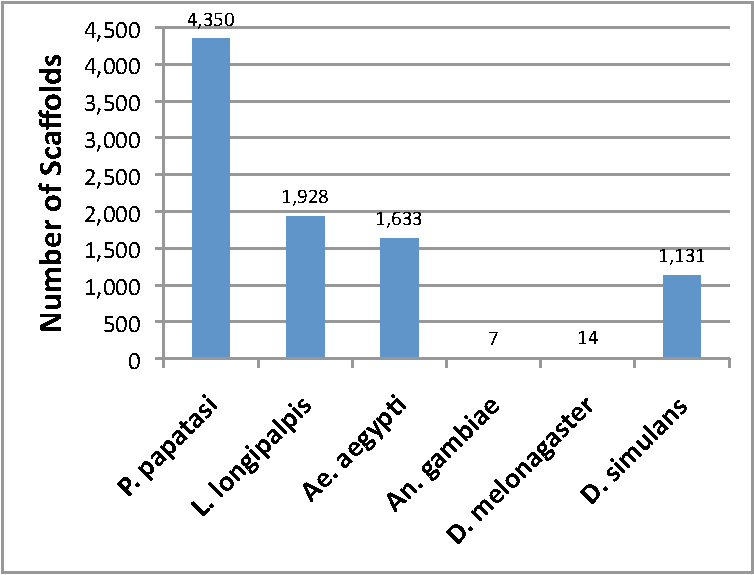
\includegraphics[width=\textwidth]{figures/synteny/scaffold_counts.pdf}
    \caption{Number of Scaffolds}
    \label{fig:number-scaffolds}
  \end{subfigure}
  ~
  \begin{subfigure}[b]{0.45\textwidth}
    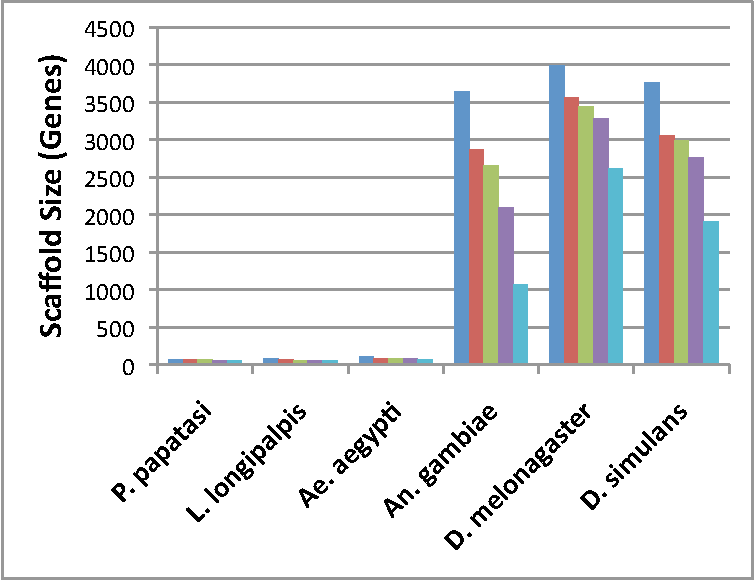
\includegraphics[width=\textwidth]{figures/synteny/top5_scaffold_sizes.pdf}
    \caption{Top 5 Scaffold Sizes (Genes)}
  \end{subfigure}
  ~
  \begin{subfigure}[b]{0.45\textwidth}
    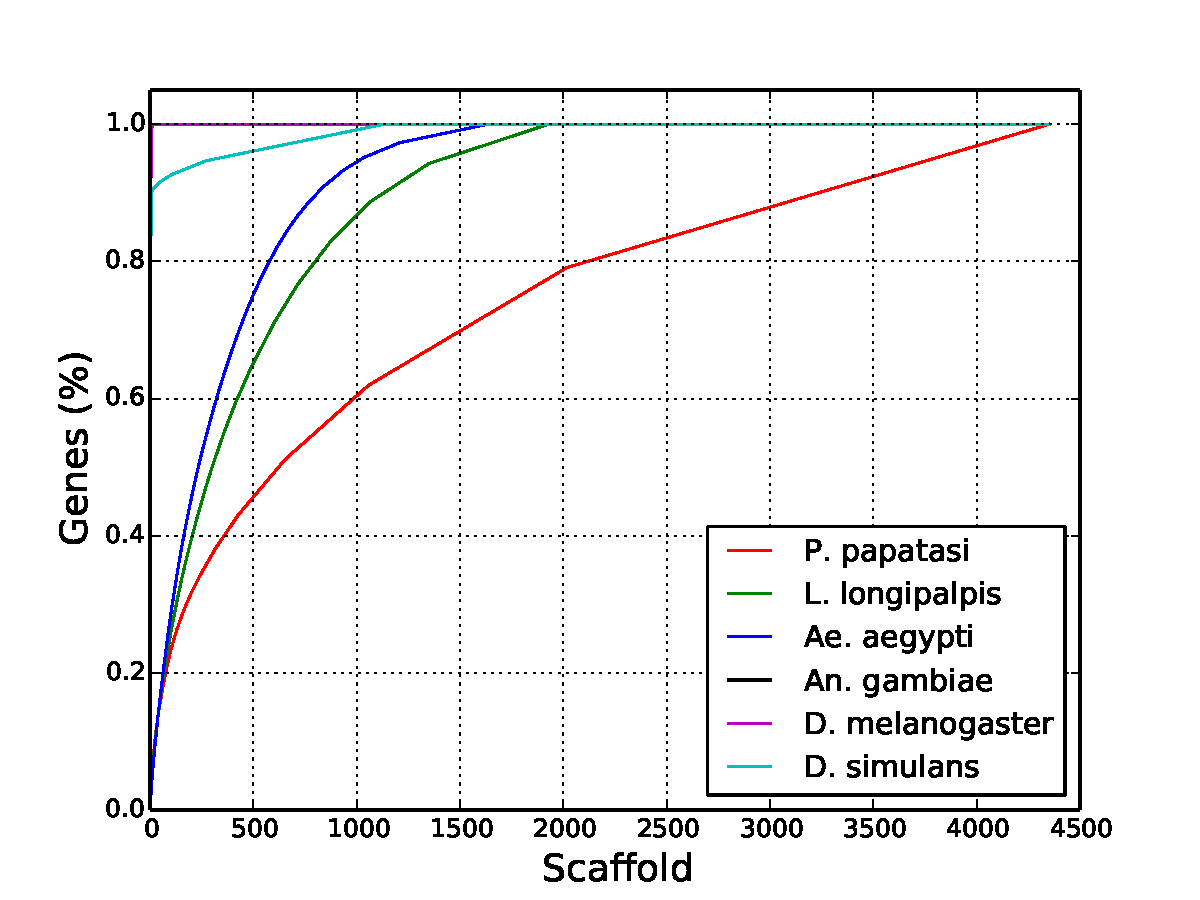
\includegraphics[width=\textwidth]{figures/synteny/gene_scaffold_cdf.pdf}
    \caption{Scaffold Genes CDF}
  \end{subfigure}
  \label{fig:scaffolds}
\end{figure}


\begin{table}[H]
  \centering
  \caption{SCAFFOLD SIZE STATISTICS}
  \begin{tabular}{c c c c c c} \hline
    \emph{Species} & \emph{Scaffolds} & \emph{Genes} & \emph{Average Size} & \emph{Median Size} & \emph{Maximumum Size} \\ \hline
    \emph{Ae. aegypti} & 1,633 & 15,797 & 9.7 & 5 & 104 \\
    \emph{An. gambiae} & 7 & 12,843 & 1834.7 & 2093 & 3,684 \\
    \emph{D. melonagaster} & 14 & 17,294 & 1235.3 & 74 & 3,991 \\ 
    \emph{D. simulans} & 1,131 & 16,196 & 14.3 & 1 & 3,767 \\ 
    \emph{L. longipalpis} & 1,928 & 10,100 & 5.2 & 1 & 73\\
    \emph{P. papatasi} & 4,350 & 11,164 & 2.6 & 1 & 84
  \end{tabular}
  \caption*{Size statistics for the scaffolds are given in numbers of genes.}
  \label{tab:scaffold-sizes}
\end{table}

\subsection{Conservation of Gene Order (Synteny)}
Rearrangements of chromosomes are rare events and tend to happen in a block-wise fashion that mainly preserves the local order of genes on the chromosome. Thus, even after long periods of divergence between species, synteny blocks, defined as conserved runs of consecutive orthologous genes, remain discernible \cite{Heger2007}.  The presence of synteny can be used to infer evolutionary relationships between organisms' genomes at a macroscopic level, complementing analyses such as gene family expansions and reductions and changes within pairs of orthologous genes \cite{Zdobnov2002,Zdobnov2007}.

We did not observe the presence of macrosynteny between the \emph{L. longipalpis} and \emph{P. papatasi} genomes (Figure~\ref{fig:synteny-dotplots-sandflies}).  Synteny analysis is dependent on the completeness of genome assemblies \cite{Heger2007}; the sizes of synteny blocks are naturally bounded by the size of the largest scaffolds (73 genes for \emph{L. longipalpis} and 84 genes for \emph{P. papatasi}). Macrosynteny was also absent in the comparison of \emph{An. gambiae} and \emph{D. melanogaster}, whose genome assemblies are complete to the level of chromosomes but present between the \emph{D. melanogaster} and \emph{D. simulans} (Figure~\ref{fig:synteny-dotplots-drosophila}), which are more closely-related than any other pair of species we've analyzed. There simply may not be macrosynteny given the high rate of genome shuffling observed in insect genomes and the evolutionary distances of the species under comparison. Comparative studies of synteny and gene order between insect genomes (e.g., \emph{Drosophila}) have indicated significant levels of genome shuffling, more so than observed in fish and humans \cite{Ranz2001,Zdobnov2002,Zdobnov2007}.

\begin{figure}[H]
  \centering
  \caption{QUALITATIVE ANALYSIS OF MACROSYNTENY}
  \begin{subfigure}[b]{0.45\textwidth}
    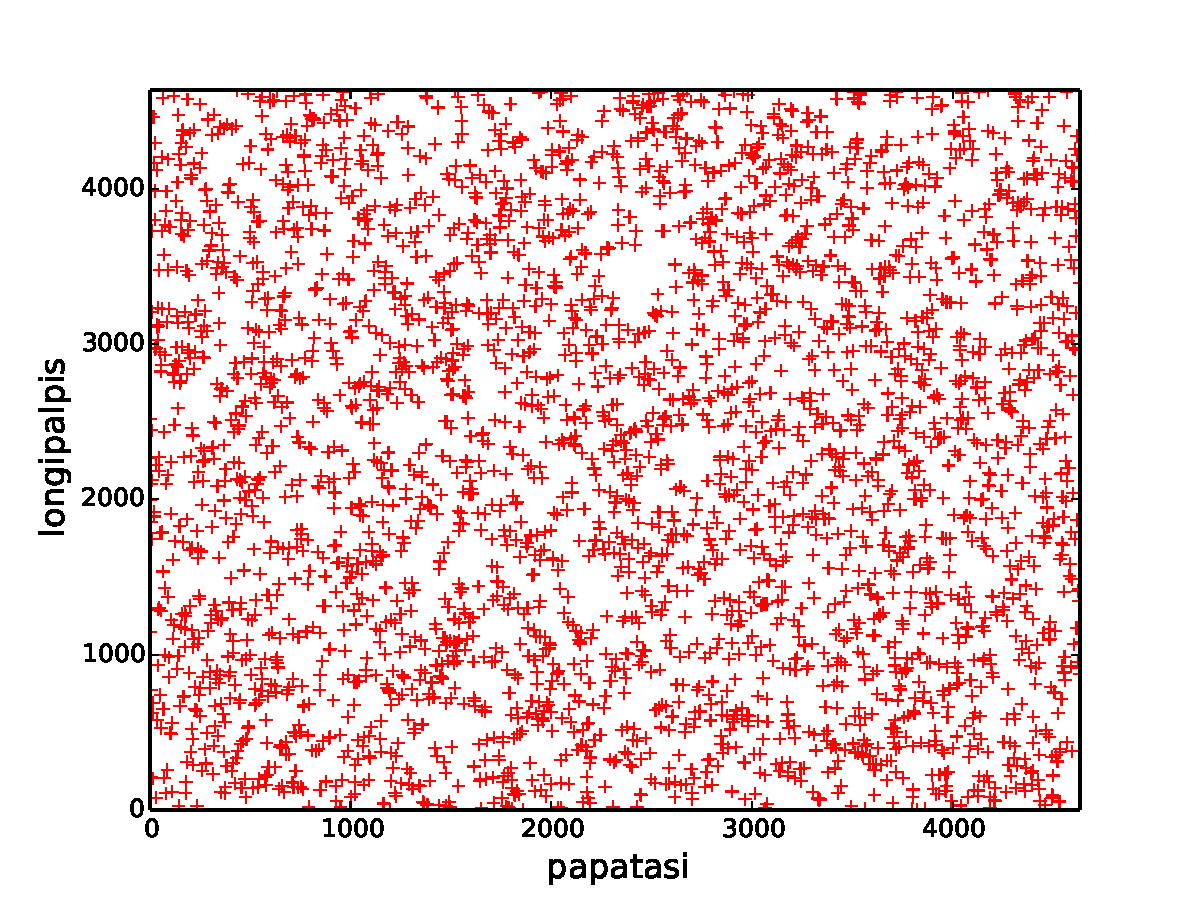
\includegraphics[width=\textwidth]{figures/synteny/papatasi_longipalpis_plot}
    \caption{\emph{L. longipalpis} vs. \emph{P. papatasi}}
    \label{fig:synteny-dotplots-sandflies}
  \end{subfigure}
  \\
  \begin{subfigure}[b]{0.45\textwidth}
    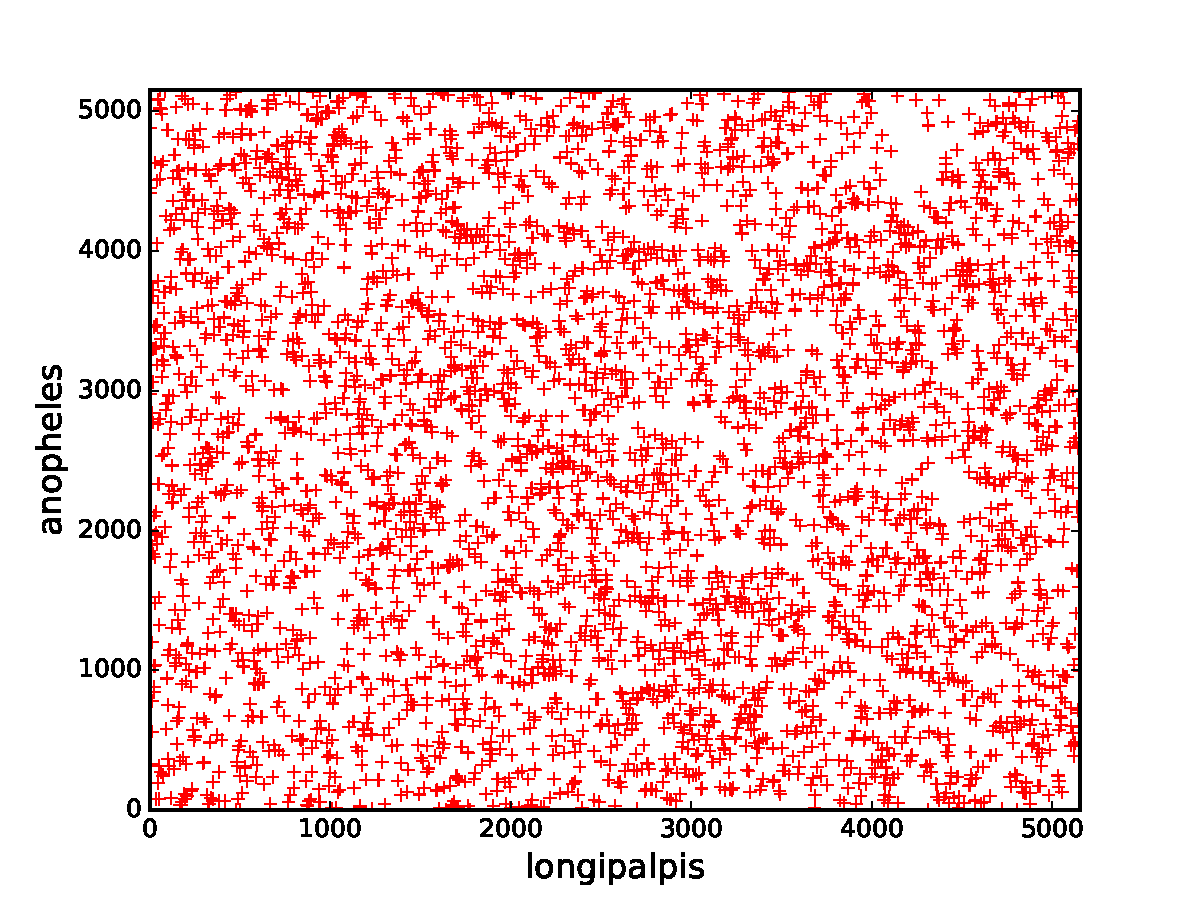
\includegraphics[width=\textwidth]{figures/synteny/longipalpis_anopheles_plot}
    \caption{\emph{L. longipalpis} vs. \emph{An. gambiae}}
    \label{fig:synteny-dotplots-longipalpis-anopheles}
  \end{subfigure}
  ~
  \begin{subfigure}[b]{0.45\textwidth}
    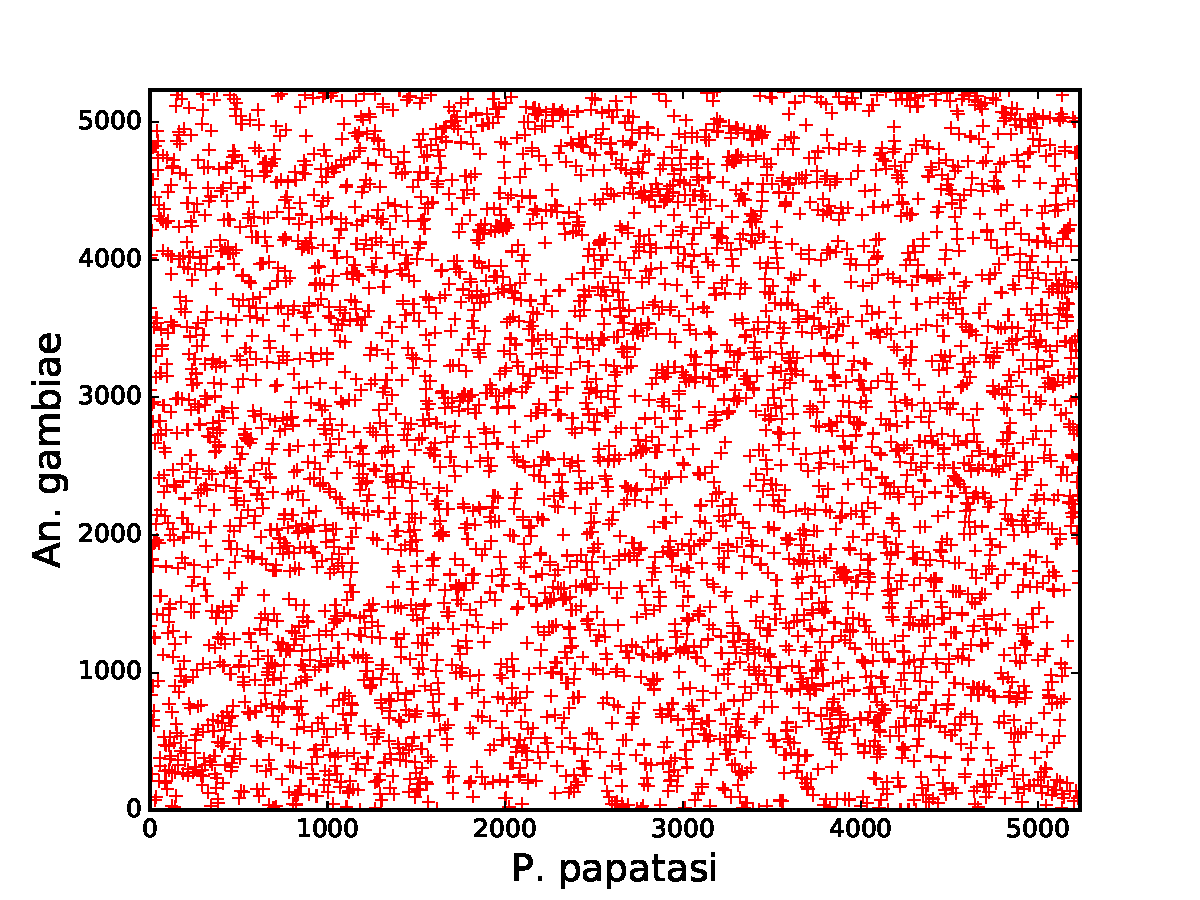
\includegraphics[width=\textwidth]{figures/synteny/papatasi_anopheles_plot}
    \caption{\emph{P. papatasi} vs. \emph{An. gambiae}}
    \label{fig:synteny-dotplots-papatasi-anopheles}
  \end{subfigure}
  ~
  \begin{subfigure}[b]{0.45\textwidth}
    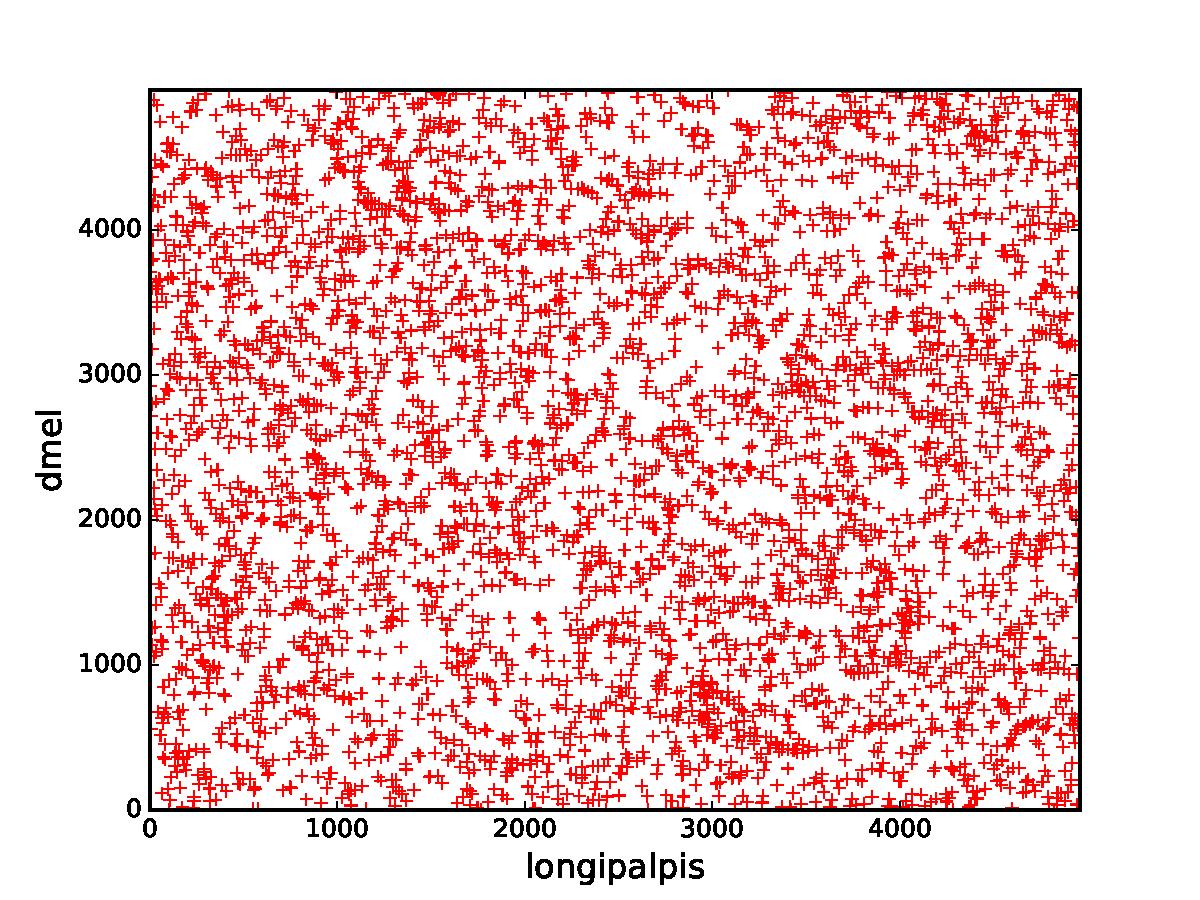
\includegraphics[width=\textwidth]{figures/synteny/longipalpis_dmel_plot}
    \caption{\emph{L. longipalpis} vs. \emph{D. melanogaster}}
    \label{fig:synteny-dotplots-longipalpis-dmel}
  \end{subfigure}
  ~
  \begin{subfigure}[b]{0.45\textwidth}
    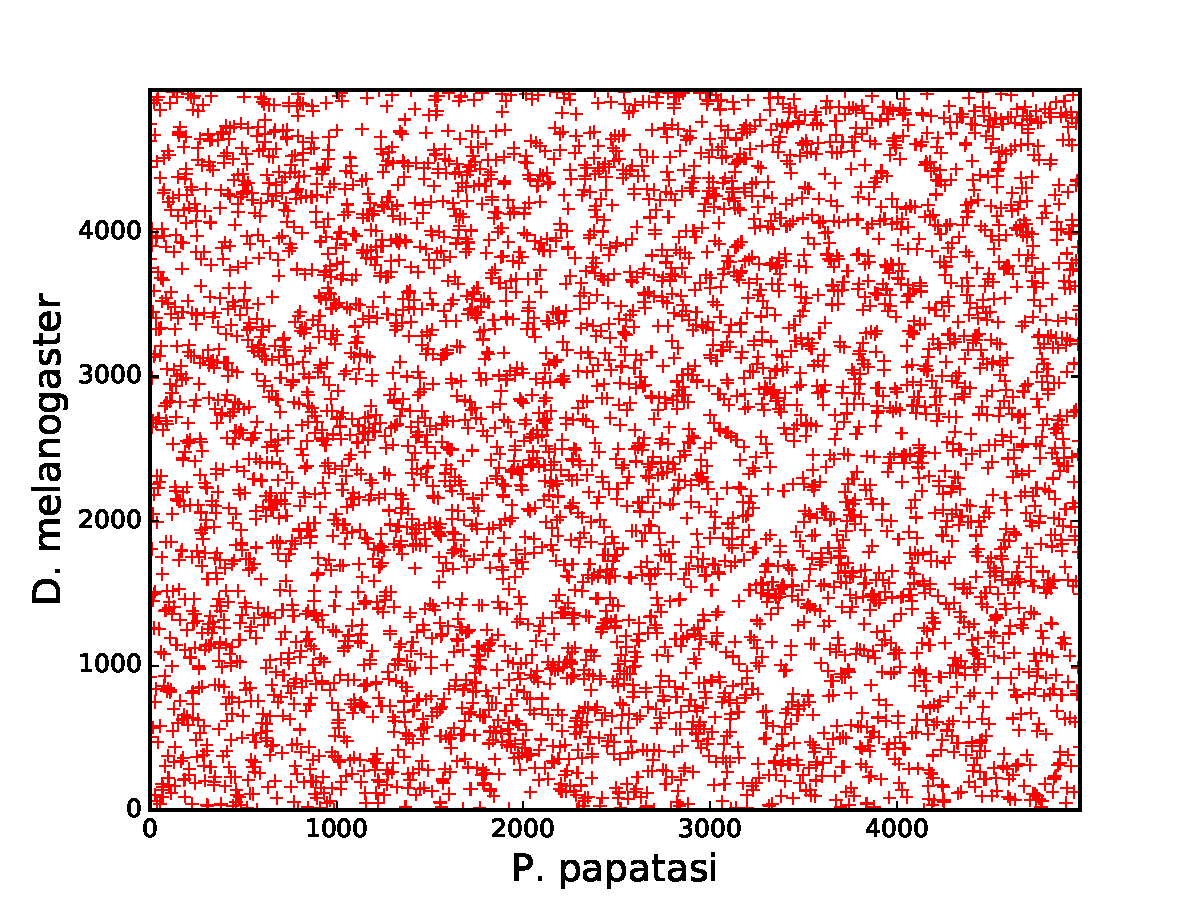
\includegraphics[width=\textwidth]{figures/synteny/papatasi_dmel_plot}
    \caption{\emph{P. papatasi} vs. \emph{D. melanogaster}}
    \label{fig:synteny-dotplots-papatasi-dmel}
  \end{subfigure}
  ~
  \begin{subfigure}[b]{0.45\textwidth}
    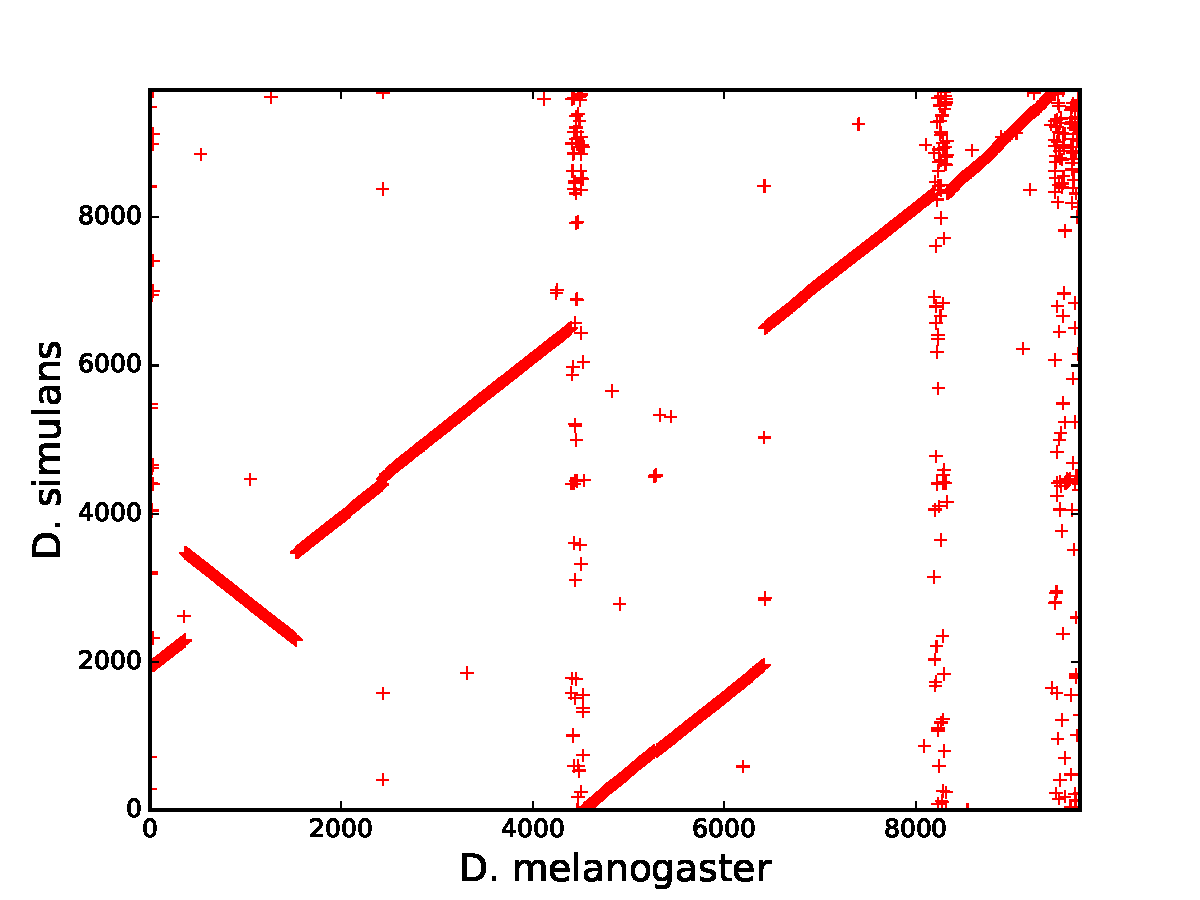
\includegraphics[width=\textwidth]{figures/synteny/dmel_dsim_plot}
    \caption{\emph{D. melanogaster} vs. \emph{D. simulans}}
    \label{fig:synteny-dotplots-drosophila}
  \end{subfigure}
  ~
  \begin{subfigure}[b]{0.45\textwidth}
    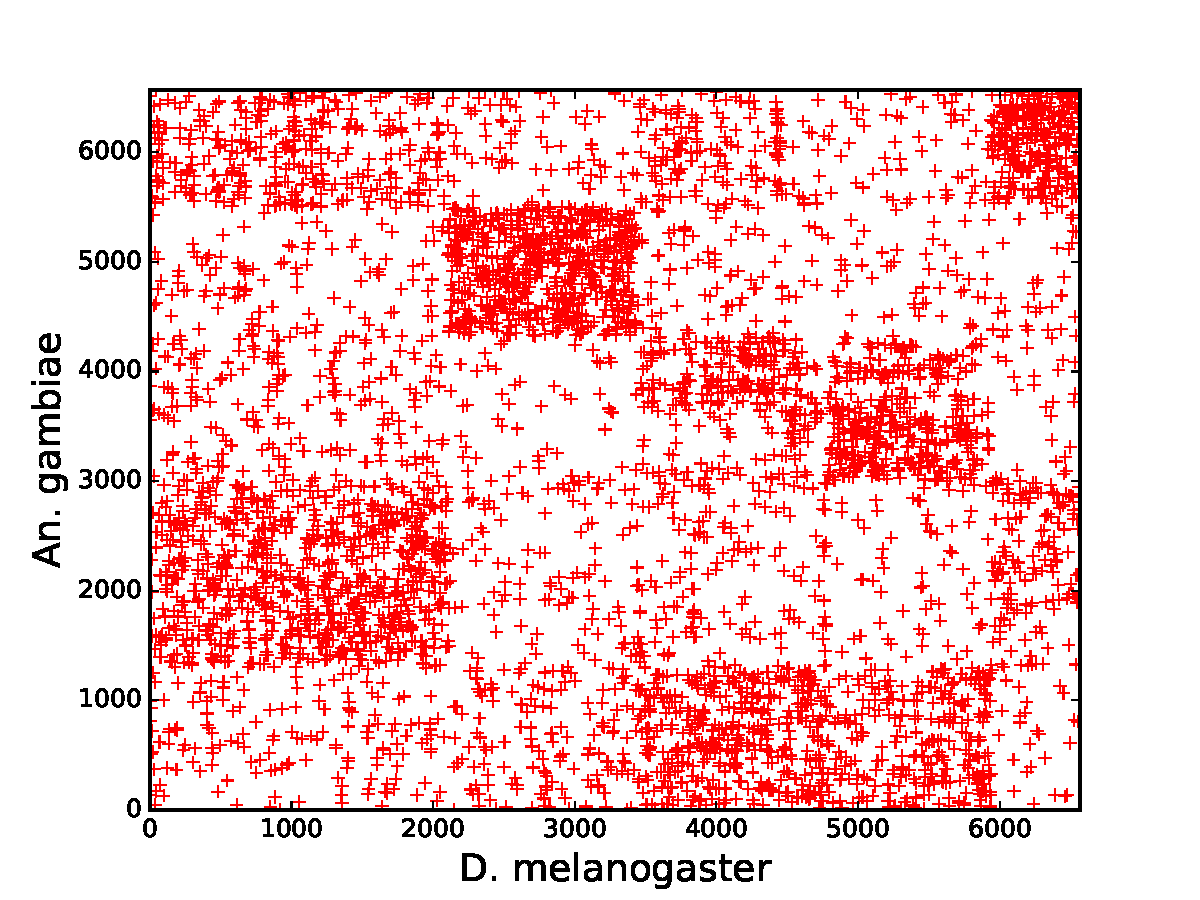
\includegraphics[width=\textwidth]{figures/synteny/dmel_anopheles_plot}
    \caption{\emph{A. gambiae} vs. \emph{D. melanogaster}}
    \label{fig:synteny-dotplots-anopheles-drosophila}
  \end{subfigure}
\label{fig:dot-plots}
\end{figure}

Microsynteny was, however, observed between the sand flies and the sand flies and \emph{An. gambiae} (Table~\ref{tab:synteny-block-stats}). Microsynteny between \emph{L. longipalpis} and \emph{P. papatasi} is on-par with the microsynteny we observed and previously reported by others for \emph{An. gambiae} and \emph{D. melonagaster}.  Between the \emph{L. longipalpis} and \emph{P. papatasi} genomes, we identified a total of 499 synteny blocks with a maximum of 24 genes, average of 4.2 genes, and a median of 3 genes. By comparison, between the genomes of \emph{An. gambiae} and \emph{D. melonagaster}, we found 1,037 synteny blocks with a maximum of 10 genes, an average of 2.5 genes, and a median of 2 genes. Previous studies of \emph{An. gambiae} and \emph{D. melonagaster} reported a similar number of synteny blocks (948) with up to 39 genes \cite{Zdobnov2002}.

\begin{table}[H]
  \centering
  \caption{MICROSYNTENY BLOCK STATISTICS}
  \begin{tabular}{c c c c c} \hline
    \emph{Species} & \emph{Count} & \emph{Average Size} & \emph{Median Size} & \emph{Maximum Size} \\ \hline
    \emph{L. longipalpis} vs. \emph{An. gambiae} & 504 & 4.3 & 3 & 39 \\
    \emph{L. longipalpis} vs. \emph{P. papatasi} & 499 & 4.2 & 3 & 24 \\
    \emph{P. papatasi} vs. \emph{An. gambiae} & 307 & 4.3 & 3 & 21 \\
    \emph{D. melanogaster} vs. \emph{D. simulans} & 243 & 41.6 & 5 & 700 \\
    \emph{D. melanogaster} vs. \emph{An. gambiae} & 1037 & 2.5 & 2 & 10
  \end{tabular}
  \caption*{Sizes are given in number of genes.}
  \label{tab:synteny-block-stats}
\end{table}

Microsynteny is more robust to genome assembly fragmentation and expected in organisms with the evolutionary distances of the sand flies and \emph{An. gambiae} \cite{Zdobnov2002}. Noncoding elements, particularly associated with gene regulation, have been found to be highly-conserved in insect microsynteny blocks, suggesting a cause for the preservation of small-scale gene order \cite{Engstrom2007}.

We annotated and analyzed the largest synteny blocks from \emph{L. longipalpis} and \emph{P. papatasi}. and a three-way comparison of \emph{An. gambiae}, \emph{L. longipalpis}, and \emph{P. papatasi}.  Four of the largest synteny blocks from \emph{L. longipalpis} and \emph{P. papatasi} contained peritrophin-like, membrane-bound or -associated, RNA regulation and synthesis, and intracellular processes genes. The largest synteny blocks between \emph{An. gambiae}, \emph{L. longipalpis}, and \emph{P. papatasi} contained genes associated with the dopamine signaling pathway and enzyme regulation, sterol homeostatis and steroid biosynthesis (Niemann-Pick type C-2), transcription regulation and protein modification, and amino acid transport and protein modification.

\subsection{Comparison of Protein Sequence Identity with $d_N$/$d_S$}
Evolutionary changes at the level of individual genes were analyzed through comparing distributions of $d_N$/$d_S$ ratios of single-copy orthologs. DNA base pairs are subject to random substitutions as organisms reproduce.  Substitutions in protein-coding open-reading frames can be divided into two types: silent mutations which do not affect the resulting amino acid sequences and non-silent mutations which do affect the resulting amino acid sequences and can affect gene function.  Silent mutations are assumed not to be under any sort of selection process, correlating with an organism's rate of evolutionary change.  Non-silent mutations are less likely to be passed on since they may impair the function of important genes; those that are inherited either do not impact gene function or are under selection pressure as an organism adapts.

The $d_N$/$d_S$ ratio measures the rate of substitutions at silent sites ($d_S$), which are presumed neutral, to the rate of substitutions at non-silent sites ($d_N$) \cite{Kryazhimskiy2008}. Genes with $d_N$/$d_S$ $>$ 1 have non-silent substitutions at a higher rate than the background rate of the organism's evolutionary change would suggest.  As such, these genes are assumed to be under positive selection pressure.  Genes with $d_N$/$d_S$ $<1$ have fewer non-silent substitutions, suggesting negative selection pressure and greater conservation in their sequences.

We analyzed $d_N$/$d_S$ ratios between single-copy orthologs in pairwise comparisons of the sand flies \emph{L. longipalpis} and \emph{P. papatasi}, mosquito \emph{An. gambiae}, and fruit fly \emph{D. melanogaster}.  The distributions of $d_N$/$d_S$ ratios are given in Figure~\ref{fig:dnds-distr}.  Except for the comparison between \emph{L. longipalpis} and \emph{P. papatasi}, the distributions are remarkedly similar.

\begin{figure}[H]
  \centering
  \caption{DISTRIBUTION OF $d_N$/$d_S$ VALUES}
  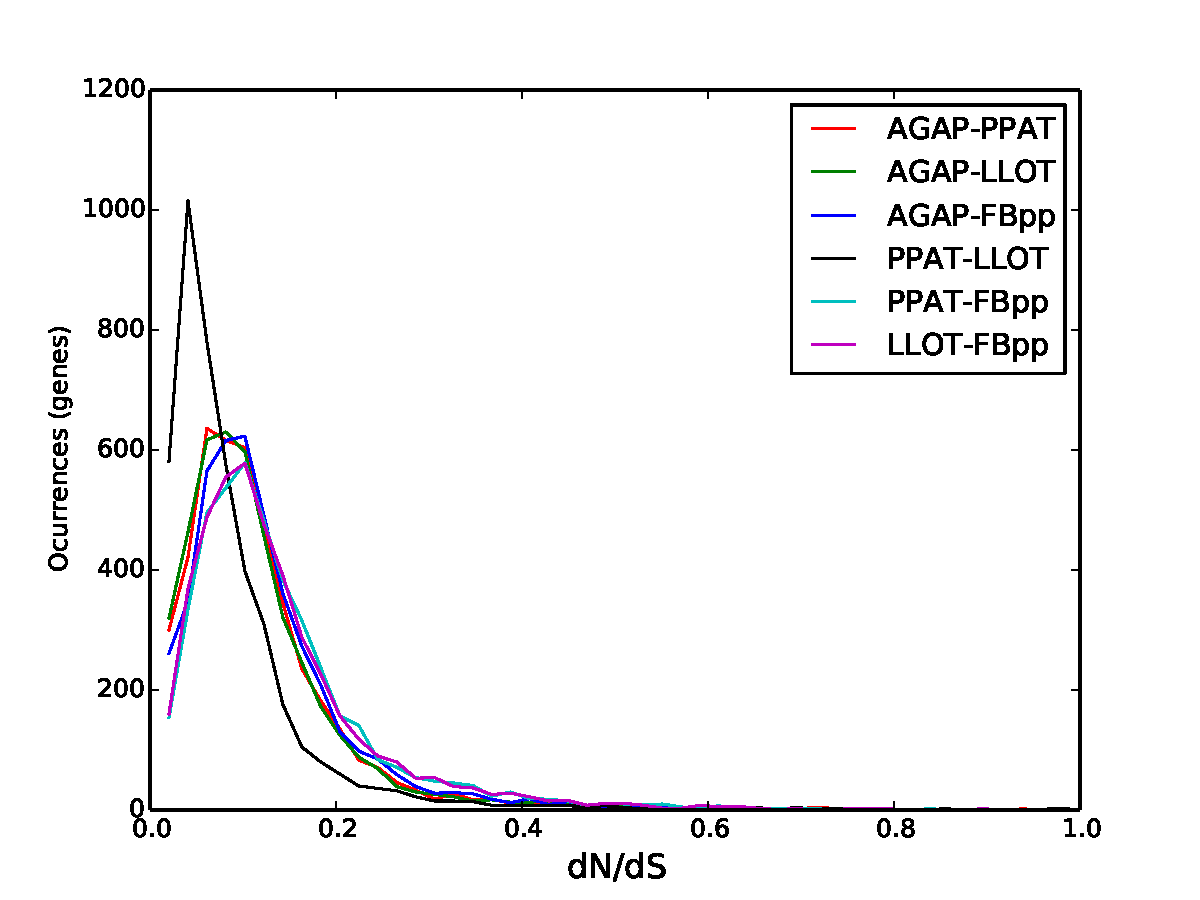
\includegraphics[width=0.75\textwidth]{figures/ka_ks/dN_dS}
  \label{fig:dnds-distr}
\end{figure}


The $d_N$/$d_S$ distribution for single-copy orthologs from \emph{L. longipalpis} and \emph{P. papatasi} is skewed towards zero when compared with distributions with and between \emph{An. gambiae} and \emph{D. melanogaster}.  The smaller $d_N$/$d_S$ values indicate fewer non-silent substitutions relative to the number of silent substitutions.  The smaller values could be a result of the shorter evolutionary distance between \emph{L. longipalpis} and \emph{P. papatasi} versus any other pair of species we compared.  However, we also found, in line with the fragmentation of the genome assemblies, that many gene models are shorter than their orthologs in other species, indicating that the gene models may not be complete (results not shown).  Thus, the lower $d_N$/$d_S$ values could also caused by truncated gene models that contain only the most conserved segments of genes.

\subsection{Differential Gene Expression in Sugar-Fed, Blood-Fed, and Infected Blood-Fed \emph{L. longipalpis} Females}
RNASeq differental gene expression data was collected from \emph{L. longipalpis} females 6, 24, and 144 hours after being fed sugar, bloodmeals, and bloodmeals infected with the Leishmaniasis parasite, \emph{Leishmania major}.  We identified approximately 3,000 to 4,500 genes with statistically-significant differences in expression between blood-fed and sugar-fed females over the three time points (see Table~\ref{tab:stat-sig-genes}).  Fewer genes (about 250 to 670) had statistically-significantly differences in expression when compared between blood-fed and infected blood-fed females.

\begin{table}[H]
  \centering
  \caption{\uppercase{Number of Genes with Statistically-Significant Differential Expression}}
  \begin{tabular}{c c c} \hline
  \emph{Time Point} & \emph{Blood Fed vs Sugar Fed} & \emph{Infected Blood Fed vs Blood Fed} \\ \hline
  6H & 3,111 & 271 \\
  24H & 4,120 & 658 \\
  144H & 4,571 & 290 \\
  \end{tabular}
  \label{tab:stat-sig-genes}
\end{table}

Comparison of GO-slim term distributions yielded little insight into differences in expression between the conditions due to the overwhelming number of genes with statistically-significant differences in expression.  As such, we focused on comparing expression of genes from families and pathways associated with immunity between blood fed and infected blood fed conditions.

\subsection{Peritrophins}
Host-parasite interactions are of particular interest.  Within a few hours, a peritrophic matrix forms around the blood bolus.  The peritrophic matrix thickens and matures around 12 to 24 hours, depending on the sand fly species.  After 48 to 72 hours, the peritrophix matric structure starts to break down.  The peritrophic matrix seems to play a dual role with respect to \emph{Leishmania} development: the peritrophic matrix protects the parasite against attack by proteolytic proteins at the beginning of digestion yet becomes a barrier to parasite escape when mature \cite{Pimenta1997,Dostalova2012}.

We analyzed differences in expression of peritrophins between sugar-fed and blood-fed conditions and blood-fed and infected blood-fed conditions.  Due to data quality issues, CuffDiff only performed statistical tests on 8 of the 28 identified of the peritrophins (see Tables~\ref{tab:sandflies:stat-sig-peritrophins-sb}~and~\ref{tab:sandflies:stat-sig-peritrophins-bi}).  LuloPer4 (LLOTMP003410), LuloPer10 (LLOTMP007615), and LuloPer11 (LLOTMP002676) had no statistically-significant differences at two or more time points.

\begin{table}[H]
  \centering
  \caption{PERITROPHIN EXPRESSION (BLOOD-FED VS. SUGAR-FED)}
  \begin{tabular}{ c c c c c } \hline
    \emph{Gene} & \emph{Identifier} & \emph{6 hours} & \emph{24 hours} & \emph{144 hours} \\ \hline
    LuloPer1 & LLOTMP006497 & Yes (3.96028) & Yes (10.5884) & No \\
    LuloPer2 & LLOTMP003676 & Yes (0.41318) & Yes (1.61758) & Yes (-0.608263) \\
    LuloPer3b & LLOTMP004906 & Yes (1.32142) & Yes (0.940809) & Yes (0.603129) \\
    LuloPer32 & LLOTMP004516 & Yes (-0.985627) & Yes (2.27779) & Yes (-2.2308)
  \end{tabular}
  \caption*{Peritrophins with statistically-significant differences in expression between sugar fed and blood fed conditions. Log-fold change is given in parentheses. Positive and negative values indicate up- and down-regulation in blood fed, respectively.}
  \label{tab:sandflies:stat-sig-peritrophins-sb}
\end{table}

\begin{table}[H]
  \centering
  \caption{PERITROPHIN EXPRESSION (INFECTED BLOOD-FED VS. BLOOD-FED)}
  \begin{tabular}{ c c c c c } \hline
    \emph{Gene} & \emph{Identifier} & \emph{6 hours} & \emph{24 hours} & \emph{144 hours} \\ \hline
    LuloPer1 & LLOTMP006497 & Yes (1.2595) & Yes (0.384657) & No \\
    LuloPer2 & LLOTMP003676 & No & Yes (0.183758) & Yes (-0.684151) \\
    LuloPer3a & LLOTMP002647 & Yes (0.283665) & Yes (0.152629) & Yes (0.358638) \\
    LuloPer3b & LLOTMP004906 & Yes (-0.137809) & Yes (1.20303) & No \\
    LuloPer32 & LLOTMP004516 & Yes (1.14581) & Yes (0.612843) & No
  \end{tabular}
  \caption*{Peritrophins with statistically-significant differences in expression between blood fed and infected blood fed conditions. Log-fold change is given in parentheses. Positive and negative values indicate up- and down-regulation in infected blood fed, respectively.}
  \label{tab:sandflies:stat-sig-peritrophins-bi}
\end{table}

A previous EST (expression tag sequence) study reported increased expression of LuloPer1 (LLOTMP006497), LuloPer2 (LLOTMP003676), and LuloPer32 (LLOTMP004516) after blood feeding \cite{Jochim2008}. Similarly, we observed up-regulation of LuloPer1, LuloPer2, and LuloPer32 at 24 hours after blood-feeding, after the peritrophic matrix thickens and matures.  We also observed increased expression of LuloPer1 and LuloPer2 but decreased expression of LuloPer32 at 6 hours, prior to the maturation of the peritrophic matrix. At 144 hours, after the peritrophic matrix starts to degrade, we observed down-regulation of LuloPer2 and LuloPer32 but no change in expression of LuloPer1.

Differential expression of LuloPer1 was observed to be increased with infected blood feeding at 6 and 24 hours, in agreement with the EST data \cite{Jochim2008,Dostalova2012}.  However, while the EST data showed no significant difference in expression under infection, we observed an increase in the expression of LuloPer32 at 6 and 24 hours and LuloPer2 at 6 hours followed by a decrease in expression at 24 hours \cite{Jochim2008}.  At 144 hours, LuloPer2 was down-regulated but LuloPer1 and LuloPer32 had no change in expression.

Differential expression levels of LuloPer3a (LLOTMP002647) and LuloPer3b (LLOTMP004906) were observed in the RNASeq analysis but were not found in the EST expression analysis \cite{Jochim2008}. LuloPer3b was up-regulated in blood fed (vs sugar fed) across all three time points and down-regulated at 6 hours and up-regulated at 24 hours in infected blood fed (vs sugar fed) conditions.  Expression of LuloPer3a had no statistically-significantly difference between blood fed and sugar fed conditions but was up-regulated across all three time points under infected bood fed (vs blood fed) conditions.

The RNASeq differential expression analysis confirmed the previous EST expression analysis of LuloPer1, LuloPer2, and LuloPer32 under blood fed (vs sugar fed) conditions and LuloPer1 under infected blood fed (vs blood fed) conditions.  We found differences in the expression of LuloPer2 and LuloPer32 under infected blood fed (vs blood fed) conditions, which had not been observed previously.  We also observed previously-unreported statistically-significant differences in expression of LuloPer3b under blood-fed (vs sugar-fed) conditions and LuloPer2 and LuloPer3b under infected blood-fed (vs blood-fed) conditions. Further analysis is needed to determine the exact functions of the peritrophins and the importance of the observed expression profiles.

LuloPer1 and four peritropins without RNASeq results are located in a microsynteny block from \emph{L. longipalpis} and \emph{P. papatasi} (see Table~\ref{tab:synteny-llot-ppat-peritrophic}). As previously noted, highly-conserved noncoding elements, particularly associated with gene regulation, have been found previously in insect microsynteny blocks \cite{Engstrom2007}.  Further study of peritrophins could potentially lead to  better understanding the relationship between regulation mechanisms and microsynteny in general and the molecular mechanisms of the peritrophin's regulation specifically.

\begin{table}[H]
  \centering
  \caption{PERITROPHIN MICROSYNTENY BLOCK}
  \begin{tabular}{c c l} \hline
    \emph{L. longipalpis} & \emph{P. papatasi} & \emph{Description} \\ \hline
    LLOTMP006493 & PPATMP009348 & SCP-related protein \\
    LLOTMP006494 & PPATMP009349 & ribosomal protein S23 \\
    LLOTMP006495 & PPATMP009350 & LuloPer22 \\
    LLOTMP006496 & PPATMP009351 & LuloPer14 \\
    LLOTMP006497 & PPATMP009352 & LuloPer1 \\
    LLOTMP006498 & PPATMP009353 &  \\
    LLOTMP006499 & PPATMP009355 & LuloPer18 \\
    LLOTMP006500 & PPATMP009356 & LuloPer17
  \end{tabular}
  \caption*{Synteny block of peritrophins from \emph{L. longipalpis} vs. \emph{P. papatasi}.}
  \label{tab:synteny-llot-ppat-peritrophic}
\end{table}


\subsection{Chitinases}
The breakdown of the peritrophic matrix has been attributed to chitinases \cite{Dostalova2012}. Eleven chitinase genes have been identified in the \emph{L. longipalpis} genome. Due to data quality issues, CuffDiff could not perform statistical tests on two of the genes, cht12 like protein (LLOTMP003713) and Llcht5 (LLOTMP008303). Llcht7 (LLOTMP009389) and Llcht8 (LLOTMP003119) did not have statistically-significant differences in expression for more than one time point in comparisons of blood-fed vs sugar-fed or blood-fed vs blood-fed infected conditions.

In a comparison of blood fed to sugar fed conditions, only two of the chitinases were up-regulated: Llcht1/midgut cht (LLOTMP000006) and Llcht8 (LLOTMP003119) were up-regulated at 6 and 24 hours, with Llcht1/midgut cht up-regulated and Llcht8 down-regulated at 144 hours.  Llcht1 was previously found to be up-regulated under blood fed vs sugar fed conditions, peaking at 72 hours \cite{Ramalho-Ortigao2003}. Neither Llcht1 nor Llcht8 had statistically-significant differences in expression levels between blood-fed and blood-fed infected conditions at any time points. RNA interference knock-down of PpChit1 (an ortholog of of Llcht1) in \emph{P. papatasi} fed \emph{L. major}-infected bloodmeals has been observed to be associated with a significantly reduction in the number of parasites present in the midgut 120 hours after the bloodmeal \cite{Coutinho-abreu2010}, suggesting that the degradation of the PM by PpChit1 enables the escape of the parasites.  Further analysis is needed to confirm a similar role for Llcht1 in \emph{L. longipalpis}. 

Five chitinases were down-regulated under blood fed vs sugar fed conditions at all time points for which differences were statistically significant: LlIDGF4 (LLOTMP008789), LlIDGF4 (LLOTMP004095), chitinase like protein (LLOTMP006041), Llcht10 (LLOTMP006362), and Llcht2 (LLOTMP008646).  In the comparisons of blood-fed vs blood-fed infected conditions, no statistically-significant differences in expression were observed for LlIDGF4 (LLOTMP008789) and Llcht2 and CuffDiff was not able to perform statistical tests on Llcht10 for two of the time points and no statistically-significant difference was found at the third time point. LlIDGF4 (LLOTMP004095) and chitinase like protein (LLOTMP006041) were the only chitinases with statistically-significant differences in expression in blood-fed vs infected blood-fed conditions; both were up-regulated at 6 and 24 hours, while at 144 hours, chitinase like protein (LLOTMP006041) was still up-regulated but LlIDGF4 (LLOTMP004095) had no statistically-significant difference. Further work is needed to understand the the role and cause of up-regulation of LlIDGF4 (LLOTMP004095) and chitinase like protein (LLOTMP006041) in the presence of \emph{Leishmania}.

\subsection{Niemann Pick C type-2-like genes}
A three-way comparison of synteny between \emph{An. gambiae}, \emph{L. longipalpis}, and \emph{P. papatasi} revealed a block of Niemann Pick type C2-like genes (Table~\ref{tab:synteny-three-way-npc2}). In insects, NPC genes are involved with sterol (e.g., cholesterol) homeostasis and biosynthesis of ecdysteroids, insect sex and moulting hormones. In humans, mutations in either of two Niemann Pick type C (NPC) genes, \emph{NPC1} and \emph{NPC2}, cause a fatal neurogenerative disorder associated with abnormal cholesterol accumulation in cells.  Previous work on NPC 2 in \emph{D. melanogaster} found that \emph{npc2a} and \emph{npc2b}, play a redundant role such that mutations in one have little discernable effect on biology; concurrent mutations in both genes lead to mortality and apoptotic neurodegeneration \cite{Huang2007}.  \emph{npc2e} and \emph{npc2a} have also been associated with the immune defiency (Imd) pathways in \emph{D. melanogaster} \cite{Shi2012}. Studies of NPC2-like genes in \emph{Ae. aegypti} have implicated ecdysteroids in a signaling cascade linking blood meal intake with vitellogenesis \cite{Sirot2011}.  Thus, the synteny of NPC2-like genes between \emph{An. gambiae}, \emph{L. longipalpis}, and \emph{P. papatasi}, may indicate similarity in sex, moulting, immunity, and feeding pathways between sand flies and mosquitoes.

\begin{table}[H]
  \centering
  \caption{NPC2 MICROSYNTENY BLOCK}
  \begin{tabular}{c c c l} \hline
    \emph{L. longipalpis} & \emph{P. papatasi} & \emph{An. gambiae} & \emph{Description} \\ \hline
    LLOTMP001853 & PPATMP007803 & AGAP002847 & Niemann-Pick type C-2 \\
    LLOTMP001854 & PPATMP007804 & AGAP002848 & Niemann-Pick type C-2 \\
    LLOTMP001855 & PPATMP007805 & AGAP002849 & Niemann-Pick type C-2 \\
    LLOTMP001857 & PPATMP007806 & AGAP002850 & Niemann-Pick type C-2 \\
    LLOTMP001858 & PPATMP007807 & AGAP002851 & Niemann-Pick type C-2 \\
    LLOTMP001859 & PPATMP007808 & AGAP002852 & Niemann-Pick type C-2 \\
    LLOTMP001861 & & AGAP002853 & Niemann-Pick type C-2 \\
    LLOTMP001863 & & AGAP002854 & Niemann-Pick type C-2 \\
    LLOTMP001864 & & AGAP002855 & Niemann-Pick type C-2 \\
    LLOTMP001865 & & AGAP002857 & Niemann-Pick type C-2
    \end{tabular}
    \caption*{Synteny block of Niemann-Pick type C-2 genes from \emph{L. longipalpis}, \emph{P. papatasi}, and \emph{An. gambiae}.}
  \label{tab:synteny-three-way-npc2}
\end{table}

We analyzed the differential gene expression in \emph{L. longipalpis} of the Niemann Pick type C-2 (NPC2) genes found to be in synteny between \emph{An. gambiae}, \emph{L. longipalpis}, and \emph{P. papatasi}.  Two genes (LLOTMP001859 and LLOTMP001861) presented statistically-significant differences in expression. Both genes had higher expression levels in blood fed or infected blood fed individuals 24 hours compared with sugar-fed individuals; by 144 hours elapsed, the genes' expression levels were significantly reduced compared to sugar-fed individuals.  The differences in expression levels between blood fed and sugar fed individuals seems to support the involvement of NPC2-like genes in a signaling cascade linking blood meal intake with vitellogenesis as observed in \emph{Ae. aegypti} \cite{Sirot2011}.

Whereas LLOTMP001861 presented little difference in expression between blood fed and infected blood fed individuals, LLOTMP001859 had significantly higher expression levels in infected blood fed individuals at 6 and 24 hours.  \emph{npc2e} and \emph{npc2a} have also been associated with the immune defiency (Imd) pathways in \emph{D. melanogaster} \cite{Shi2012}.  Depletion of Caspar, a negative regulator of the immune deficiency (IMD) pathway, with RNA interference was previously shown to reduce population infection rates from 85\% to 45\% suggesting that the IMD pathway plays a role in frustrating infection by \emph{L. major} \cite{Telleria2012}.  The differences in expression may indicate that LLOTMP001859 plays a role in immune response to the \emph{Leishmania} parasite.


\section{Conclusion}





